\section{Evaluation}

\subsection{Implementation of Transfer Learning}

\subsection{Implementation of Siamese Network}

In this project, we implement both two loss functions with the same dataset. The dataset processing is presented in section \ref{}. 

\subsubsection{Implementation of contrastive loss}
For contrastive loss, we implement and train siamese networks using Keras and Tensorflow. The implementation can be partitioned into three steps: 1) generating image pairs, 2) construct the architecture of the siamese neural network, 3) using contrastive loss to train the model. Note that the siamese network was designed originally for the image matching task, not the image classification. Normally, it would have a distance function to compute the similarity between the two embedding vectors as the final outputs. However, our project is for the image classification problem, so we implement a single dense layer on top of that to train the embedding vectors extracted from the siamese network. In doing so, we get classification results that are similar to the transfer learning models. 

Specifically, in this project, we adopt a simple strategy to make the image pairs. The positive sample of an anchor sample is picked randomly from the same category as the anchor. On the other hand, we grab the negative sample randomly from classes that are different from the one that the anchor belongs to. Furthermore, we label the positive pairs with 1 and the positive pairs with 0. Figure \ref{fig:threesamples} shows the examples of the anchor, positive and negative samples. 

\begin{figure}[h]
  \centering
  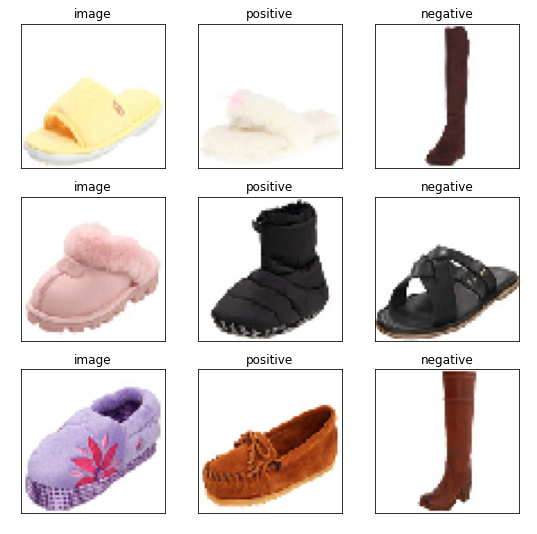
\includegraphics[width=0.9\linewidth]{figs/threesamples.png}
  \caption{Examples of anchor, positive and negative samples.}
  \label{fig:threesamples}
\end{figure}

Furthermore, we can also compute the similarity between image pairs, as shown in figure \ref{}. Note that the smaller distance between the two images means they are more similar to each other. For example, in the figure, the distance between the first pair is 0.12, and it turns out that they belong to the same class Slippers. As for the second pair, the class of left image is Slippers and the class of right image is Sandals. The distance between them is 0.56, which is much larger than the first pair, as we expected. 

\begin{figure}[h]
  \centering
  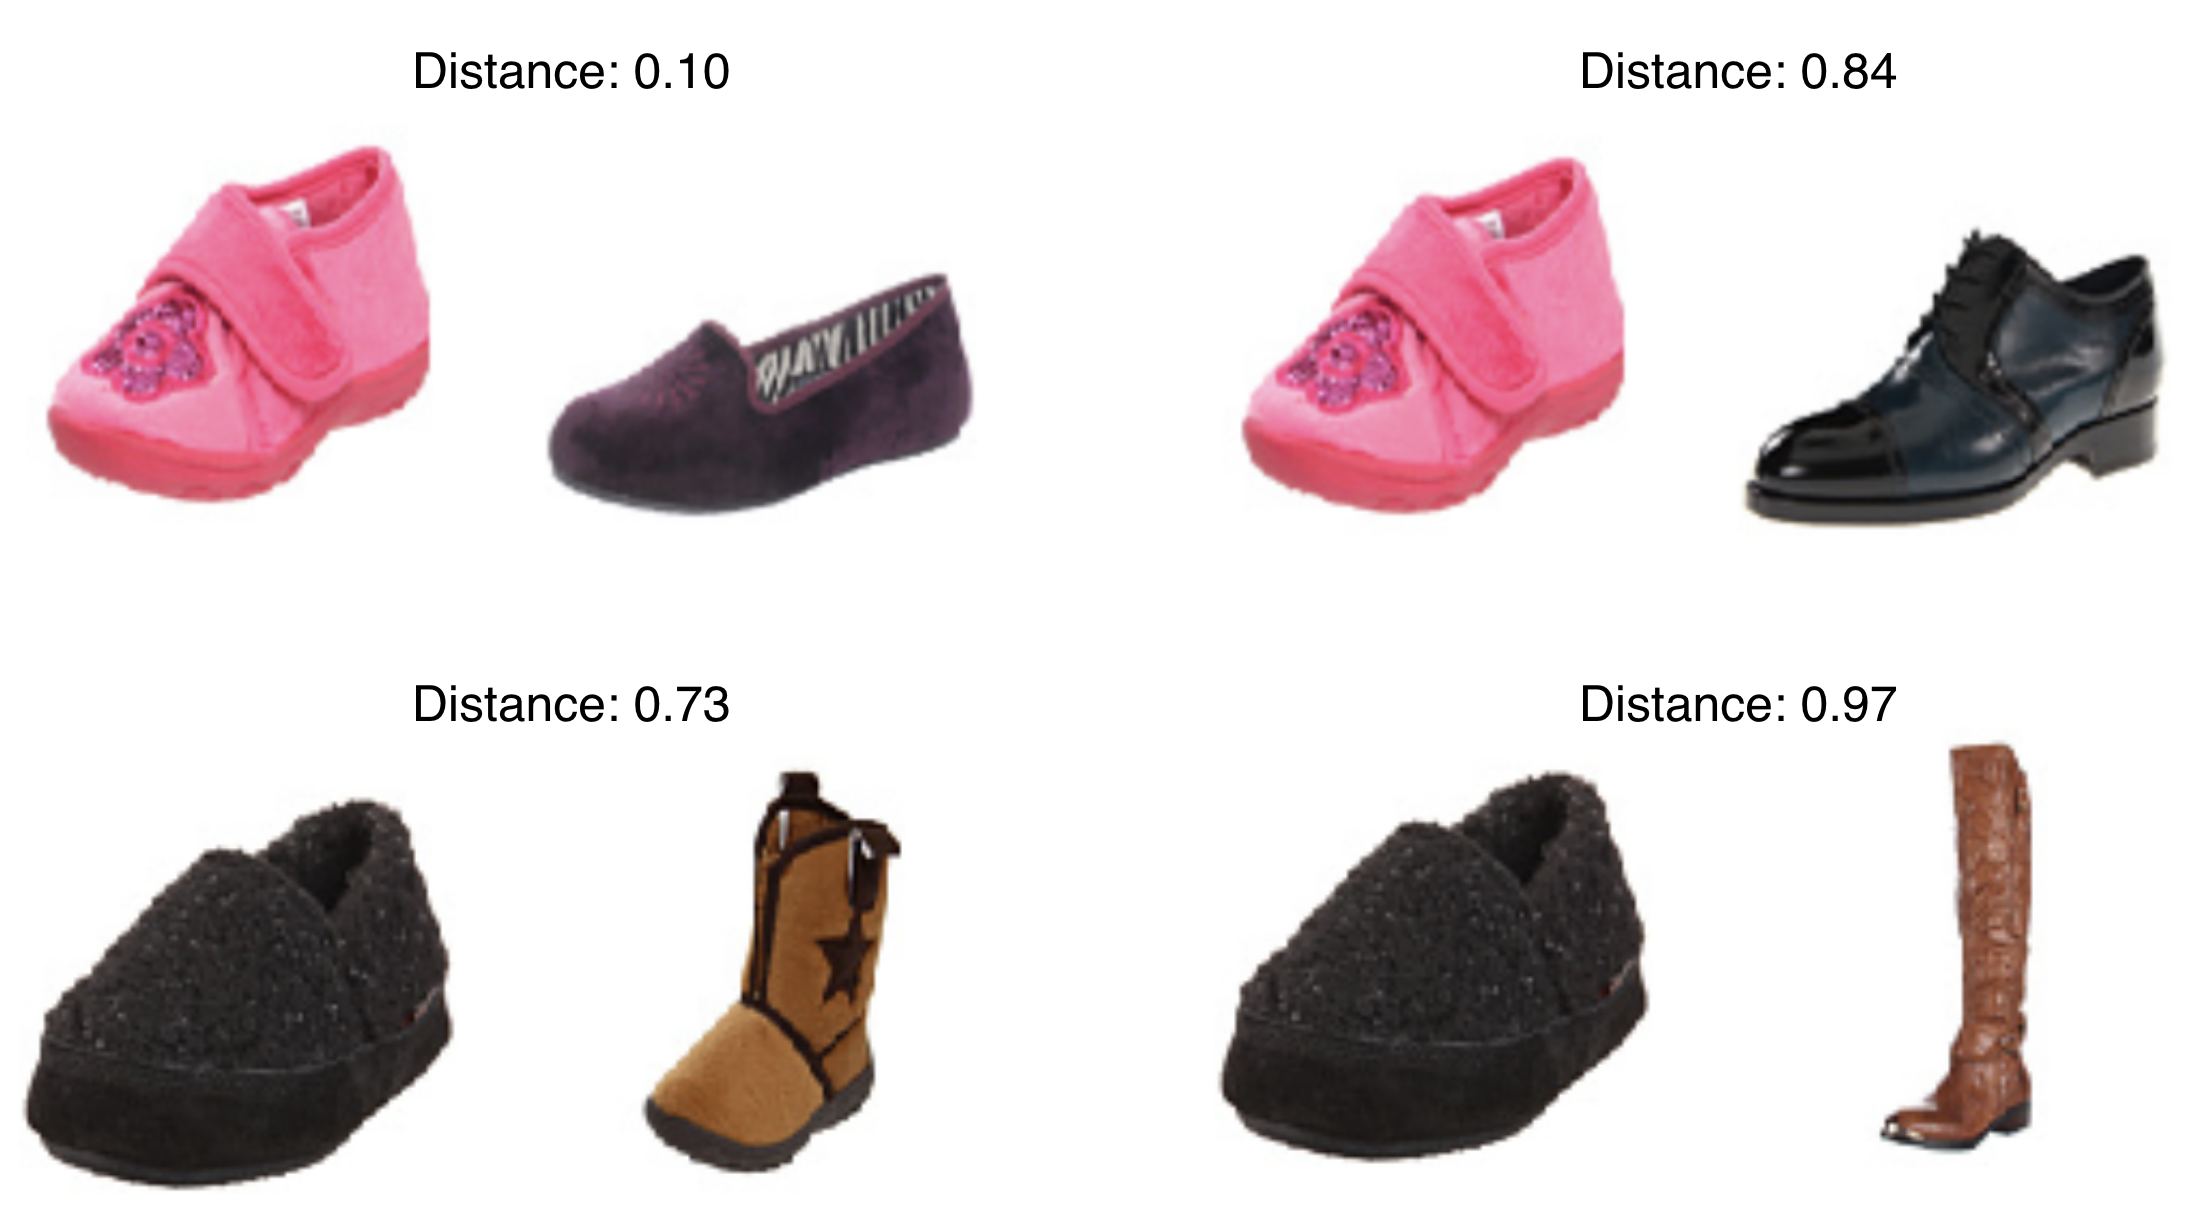
\includegraphics[width=0.5\linewidth]{figs/similarity.png}
  \caption{Examples of calculating the similarity of image pairs.}
  \label{fig:similarity}
\end{figure}

\subsubsection{Implementation of triplet loss}


\subsection{Comparison and Analysis}

In our implementation, we observe that the triplet loss a little outperforms the contrastive loss. The possible reasons could be the triplet loss tries to be less greedy than contrastive loss since the distance is a relative concept. The triplet loss tries to bring the positive sample closer while also pushing away the negative sample when compared with an anchor, as shown in the figure \ref{fig:tripletloss}. In doing so, the model can clear know if the distance between the anchor sample and positive sample is smaller than the distance between the anchor and negative one. On the other hand, the contrastive loss, only considers one pair at a time, either positive or negative, so in a sense, it is more greedy. It's hard to ensure the similar objects are close enough. 

\begin{figure}[h]
  \centering
  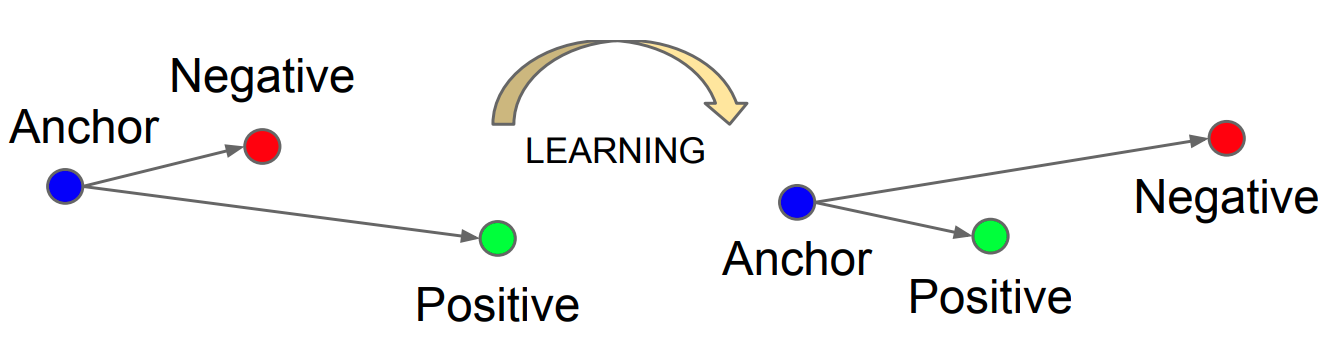
\includegraphics[width=\linewidth]{figs/tripletloss.png}
  \caption{The Triplet Loss minimizes the distance between an anchor and a positive, and maximizes the distance between the anchor and a negative.}
  \label{fig:tripletloss}
\end{figure}

